\section{}
% A 2.4-in-diameter smooth ball rotating (anticlockwise) at 500 rpm is 
% dropped in a water stream at 60℉ flowing at 4 ft/s. Determine the lift and the drag force acting on 
% the ball when it is first dropped in the water. (�%!&'# = 62.36 ()*
% +&! ; �%!&'# = 7.536 ×
% ,-"#()*
% +& ∙ �)
% Note: for smooth rotating ball �. = /$
% %
% &
% 01&'
% #.& , �2 = /(
% %
% &
% 01&'
% #.

A 2.4-in-diameter smooth ball rotating (anticlockwise) at 500 rpm is dropped in a water stream at 60$^\circ$F flowing at 4 ft/s. 
Determine the lift and the drag force acting on the ball when it is first dropped in the water. 
($\rho$ = 62.36 lbm/ft$^3$, $\mu$ = 7.536 $\times$ 10$^{-4}$ lb/(ft$\cdot$s))
Note: for smooth rotating ball $C_D = \frac{F_D}{\frac{\pi}{8} \rho V^2 D^2}$, $C_L = \frac{F_L}{\frac{\pi}{8} \rho V^2 D^2}$.

Find the Reynolds number:
\begin{align*}
    Re &= \frac{\rho V D}{\mu} \\
       &= \frac{(62.36)(4)(2.4/12)}{7.536 \times 10^{-4}} \\
       &= 6.62 \times 10^4
\end{align*}

Nondimensional rate of rotation is 
\begin{align*}
    \frac{1}{2}\omega D/V &= \frac{1}{2} 500 \times 2\pi/60} \frac{2.4}{12\times 4} \\
    &= 1.309
\end{align*}

From Figure \ref{fig:Q2Graph}, $C_D = 0.55$ and $C_L = 0.35$. Then
\begin{figure}[h]
    \centering
    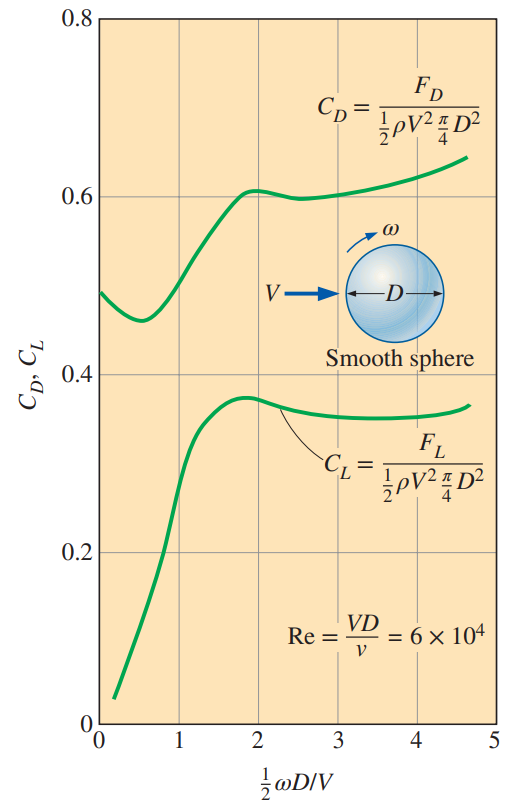
\includegraphics[width=0.5\linewidth]{Questions/Figures/Q2Graph.png}
    \caption{Drag and lift coefficients for a smooth rotating sphere with nondimensional rate of rotation Re = $6 \times 10^4$}
    \label{fig:Q2Graph}
\end{figure}

\begin{align*}
    F_L &= \frac{\pi}{8} \rho V^2 D^2 C_L \\
        &= \frac{\pi}{8} (62.36) (4)^2 (2.4/12)^2 (0.35) \times \frac{1}{32.174}
        \boxed{0.1705 \text{ lbf}} \\
    F_D &= \frac{\pi}{8} \rho V^2 D^2 C_D \\
        &= \frac{\pi}{8} (62.36) (4)^2 (2.4/12)^2 (0.55) \times \frac{1}{32.174}
        \boxed{0.268 \text{ lbf}}
\end{align*}